% =====================================================================
%  BÀI BÁO TÓM TẮT ĐỀ TÀI (2 cột, 6 đến 8 trang)
%  Theo "Hướng dẫn cách trình bày bài viết đăng trên Tạp chí Khoa học Giáo dục Kỹ thuật" (HCMUTE):
%  A4, Times 12, lề trên/dưới 1,5 cm, trái 2,5 cm, phải 2 cm, 2 cột cách nhau 0,5 cm,
%  dãn đoạn 6 pt, dòng đơn; đề mục chính IN HOA ĐẬM, đề mục phụ thường đậm;
%  tựa Việt in hoa đậm, cỡ 14; tác giả đậm, đơn vị nghiêng; chỉ có tóm tắt tiếng Việt;
%  tài liệu tham khảo đánh số theo thứ tự trích dẫn.
%  Biên dịch (2 lần): pdflatex -jobname="24119068_Huỳnh Lê Thành Nhân_Report" vieedge_paper.tex
% =====================================================================
\documentclass[a4paper,12pt,twocolumn]{article}
\usepackage[T5]{fontenc}
\usepackage[utf8]{inputenc}
\usepackage[vietnamese]{babel}
\usepackage{mathptmx}
\usepackage[scaled=.92]{helvet}
\usepackage[a4paper,top=1.5cm,bottom=1.5cm,left=2.5cm,right=2.0cm,footskip=.75cm]{geometry}
\usepackage{graphicx,booktabs,array,xcolor,amsmath,amssymb,microtype,tikz,enumitem,fancyhdr}
\usepackage[font=small,labelfont=bf,labelsep=period,skip=4pt]{caption}
\usepackage[hidelinks,pdftitle={VieEdge-Voice: Trợ lý hỏi đáp bằng giọng nói tiếng Việt chạy hoàn toàn offline trên thiết bị biên},pdfauthor={Huỳnh Lê Thành Nhân (24119068), Nguyễn Đoàn Hoàng Ngân (24119064)},unicode]{hyperref}
\usepackage{stfloats}
\usepackage{balance}
\usepackage{titlesec}
\usetikzlibrary{arrows.meta,positioning,calc}
% Thông tin chung cho bài báo và poster: sửa một chỗ ở đây.
\newcommand{\tenviet}{VieEdge-Voice: Trợ lý hỏi đáp bằng giọng nói tiếng Việt chạy hoàn toàn offline trên thiết bị biên}
\newcommand{\TENVIET}{VIEEDGE-VOICE: TRỢ LÝ HỎI ĐÁP BẰNG GIỌNG NÓI TIẾNG VIỆT CHẠY HOÀN TOÀN OFFLINE TRÊN THIẾT BỊ BIÊN}
\newcommand{\tenanh}{VieEdge-Voice: a fully offline Vietnamese voice question-answering assistant on edge devices}
\newcommand{\svmot}{Huỳnh Lê Thành Nhân}
\newcommand{\mssvmot}{24119068}
\newcommand{\svhai}{Nguyễn Đoàn Hoàng Ngân}
\newcommand{\mssvhai}{24119064}
\newcommand{\emailmot}{24119068@student.hcmute.edu.vn}
\newcommand{\truong}{Trường Đại học Công nghệ Kỹ thuật Thành phố Hồ Chí Minh}
\newcommand{\khoa}{Khoa Đào tạo tiên tiến}
\definecolor{xanhute}{HTML}{0272BC}
\definecolor{doute}{HTML}{D3202A}
\definecolor{dam}{HTML}{0B3C78}

\graphicspath{{../figures/}}
\addto\captionsvietnamese{\renewcommand{\figurename}{Hình}\renewcommand{\tablename}{Bảng}\renewcommand{\refname}{}}
\setlength{\columnsep}{0.5cm}
\setlength{\parindent}{0pt}
\setlength{\parskip}{6pt}
\setlength{\textfloatsep}{8pt plus 2pt minus 2pt}
\setlength{\floatsep}{8pt plus 2pt minus 2pt}
\setlength{\dbltextfloatsep}{8pt plus 2pt minus 2pt}
\setlength{\abovecaptionskip}{4pt}
\pagestyle{fancy}\fancyhf{}\renewcommand{\headrulewidth}{0pt}
\fancyfoot[C]{\small\thepage}
\titleformat{\section}{\normalfont\normalsize\bfseries}{\thesection.}{.4em}{\MakeUppercase}
\titlespacing*{\section}{0pt}{10pt}{2pt}
\titleformat{\subsection}{\normalfont\normalsize\bfseries}{\thesubsection.}{.4em}{}
\titlespacing*{\subsection}{0pt}{6pt}{0pt}
\setlist{itemsep=1pt,topsep=-3pt,parsep=0pt,leftmargin=1.5em}
\newcolumntype{R}[1]{>{\raggedleft\arraybackslash}p{#1}}
\newcolumntype{L}[1]{>{\raggedright\arraybackslash}p{#1}}
\newcommand{\vso}[1]{\ensuremath{#1}}
\hyphenpenalty=1500 \emergencystretch=1.2em
\sloppy

\begin{document}
\twocolumn[{%
\noindent
\includegraphics[height=8.5mm]{logo_hcmute.png}\hfill
\raisebox{3mm}{\small\itshape Báo cáo tóm tắt đề tài dự thi}\par\vspace{5pt}
\begin{center}
{\fontsize{14}{17}\selectfont\bfseries \TENVIET\par}
\end{center}
\vspace{3pt}
\begin{flushright}\setlength{\parskip}{0pt}
\textbf{\svmot}$^{*}$ (MSSV \mssvmot), \textbf{\svhai} (MSSV \mssvhai)\\
\textit{\khoa, \truong}
\end{flushright}
\vspace{1pt}
\noindent\textbf{TÓM TẮT}\par
\noindent Trợ lý giọng nói phổ biến hiện nay phụ thuộc đám mây, nên ngừng hoạt động khi mất mạng và phải gửi giọng nói của người dùng ra ngoài. Chúng tôi đặt câu hỏi: một thiết bị biên có thể nghe, hiểu và trả lời bằng tiếng Việt, không Internet, đủ nhanh để hội thoại hay không. VieEdge-Voice là đường ống offline trọn vòng gồm nhận dạng giọng nói Zipformer, tra cứu Wikipedia cục bộ, mô hình ngôn ngữ lớn lượng tử hoá và tổng hợp tiếng nói Piper, triển khai trên Raspberry Pi 5 với Yocto PREEMPT\_RT và trên ứng dụng Android dùng NPU của Galaxy Z Fold7. Tỉ lệ lỗi từ trên VIVOS là 0,041. Trên điện thoại, mô hình 2 tỉ tham số bắt đầu đọc câu trả lời thật sau 1,53\,s tính từ lúc người dùng nói xong, kể cả khi bật tra cứu; câu hỏi có sẵn đi đường nhanh trên Pi được trả lời sau 0,52\,s. So sánh cùng phần cứng cho thấy Yocto-RT giảm đỉnh jitter của lõi âm thanh 19 đến 28\% nhưng không làm suy luận nhanh hơn. Cho kịch bản mất sóng khi thiên tai, 42 thẻ sơ cứu và ứng phó viết sẵn có nguồn chọn đúng thẻ cho 79 trên 84 câu thử độc lập, để mô hình không phải tự sinh lời khuyên y tế. Các đo đạc dùng câu viết sẵn và giọng đọc tổng hợp; đánh giá với giọng người là bước tiếp theo.

\vspace{2pt}
\noindent\textbf{Từ khóa:} trợ lý giọng nói; tiếng Việt; thiết bị biên; NPU; mô hình ngôn ngữ lớn; PREEMPT\_RT.

\vspace{8pt}
}]
\thispagestyle{fancy}

\section{Giới thiệu}
Trong hội thoại, người nói giữ khoảng lặng giữa hai lượt lời rất ngắn và tránh để nó kéo dài, với chênh lệch giữa các ngôn ngữ chỉ trong khoảng 250\,ms quanh mức trung bình~\cite{stivers}. Trợ lý giọng nói vì vậy bị đánh giá bằng thời gian chờ, không chỉ bằng độ đúng. Các hệ thống chạy trên đám mây giải quyết tốc độ bằng máy chủ lớn, đổi lại cần mạng và phải đưa giọng nói ra khỏi thiết bị. Mạng lại hay mất đúng lúc cần nhất: bão lũ, sạt lở cắt sóng và điện, trong khi người dân cần hỏi cách sơ cứu hay thoát hiểm ngay. Đây là kịch bản sử dụng chính của đề tài.

Đưa bài toán này xuống thiết bị biên bằng tiếng Việt vướng ba rào cản. Mô hình nhận dạng phổ thông kém trên tiếng Việt: Whisper-tiny~\cite{whisper} sai 53\% số từ trên VIVOS trong phép đo của chúng tôi, và mô hình tinh chỉnh như PhoWhisper~\cite{phowhisper} vẫn phải chọn giữa cỡ và độ chính xác. Đường ống nối tiếp cộng dồn độ trễ vì mỗi khâu chờ khâu trước~\cite{chipchat}. Mỗi nền tảng lại có giới hạn riêng: Hailo-8L chỉ nhận mạng tĩnh, CPU của Pi~5 nạp prompt chậm, còn NPU điện thoại cần chuỗi công cụ của nhà sản xuất.

MELT~\cite{melt} đánh giá LLM trên điện thoại nhưng chỉ riêng khâu LLM. ChipChat~\cite{chipchat} đạt độ trễ dưới một giây trên Mac Studio bằng thiết kế xếp tầng, trên phần cứng mạnh hơn nhiều. Chúng tôi chưa tìm thấy công bố nào đo trọn vòng tiếng Việt, từ lúc người dùng nói xong tới lúc nghe câu trả lời, trên cả máy nhúng lẫn NPU điện thoại với cùng một quy ước đo.

Đóng góp của đề tài gồm: (i) đường ống offline đo được từng chặng, chạy thật trên hai nền tảng (Mục~\ref{sec:system}); (ii) phân tích thời gian đi đâu và các biện pháp giảm độ trễ kèm phép đo bật tắt từng biện pháp (Mục~\ref{sec:latency}); (iii) so sánh Pi OS và Yocto-RT trên cùng bo mạch có kiểm định thống kê (Mục~\ref{sec:os}); (iv) so sánh CPU, GPU, NPU và các kết quả âm có đo đạc (Mục~\ref{sec:platform} và \ref{sec:negative}); (v) bộ thẻ sơ cứu và ứng phó thiên tai có nguồn, kèm bộ khớp câu hỏi được đánh giá trên tập câu độc lập (Mục~\ref{sec:safety}). Hai kết quả không thuận lợi được nêu ngay ở đây: encoder lượng tử trên Hailo-8L chưa dùng được, và hệ điều hành thời gian thực không làm LLM nhanh hơn.

\section{Hệ thống và phương pháp}\label{sec:system}
\subsection{Phần cứng}
Nền tảng nhúng là Raspberry Pi 5 8\,GB (4 lõi Cortex-A76, có dotprod, không có i8mm) gắn Hailo-8L, chạy ảnh Yocto scarthgap với kernel 6.12 PREEMPT\_RT. Nền tảng di động là Samsung Galaxy Z Fold7 (Snapdragon 8 Elite, Hexagon v79, GPU Adreno, Android 16). Sản phẩm gồm ứng dụng Android viết bằng Kotlin chạy toàn bộ đường ống ngay trên máy, có thêm chế độ dùng điện thoại làm micro và loa cho Pi qua WebSocket; ảnh Yocto dựng lại được từ cấu hình; và bảng điều khiển web hiện chữ, câu trả lời và thời gian từng chặng.

\subsection{Đường ống}
Hình~\ref{fig:arch} là lưu đồ của một lượt hỏi. Silero VAD~\cite{silero} phát hiện lời nói và ngắt câu sau 400\,ms im lặng. Zipformer~\cite{zipformer} bản tiếng Việt 30 triệu tham số~\cite{zipvi}, chạy INT8 trên CPU qua sherpa-onnx~\cite{sherpa}, chép lời thành chữ kèm điểm tin cậy; câu dưới ngưỡng tin cậy được yêu cầu nói lại. Câu hỏi sau đó tới đường nhanh hoặc tới tra cứu cộng LLM. Khối tách câu đẩy câu đầu sang tổng hợp tiếng nói ngay khi đủ số từ, văn bản được chuẩn hoá (số, ngày, đơn vị) rồi đọc bằng Piper~\cite{piper}, một bộ tổng hợp dựa trên VITS~\cite{vits}.

\begin{figure*}[t]
\centering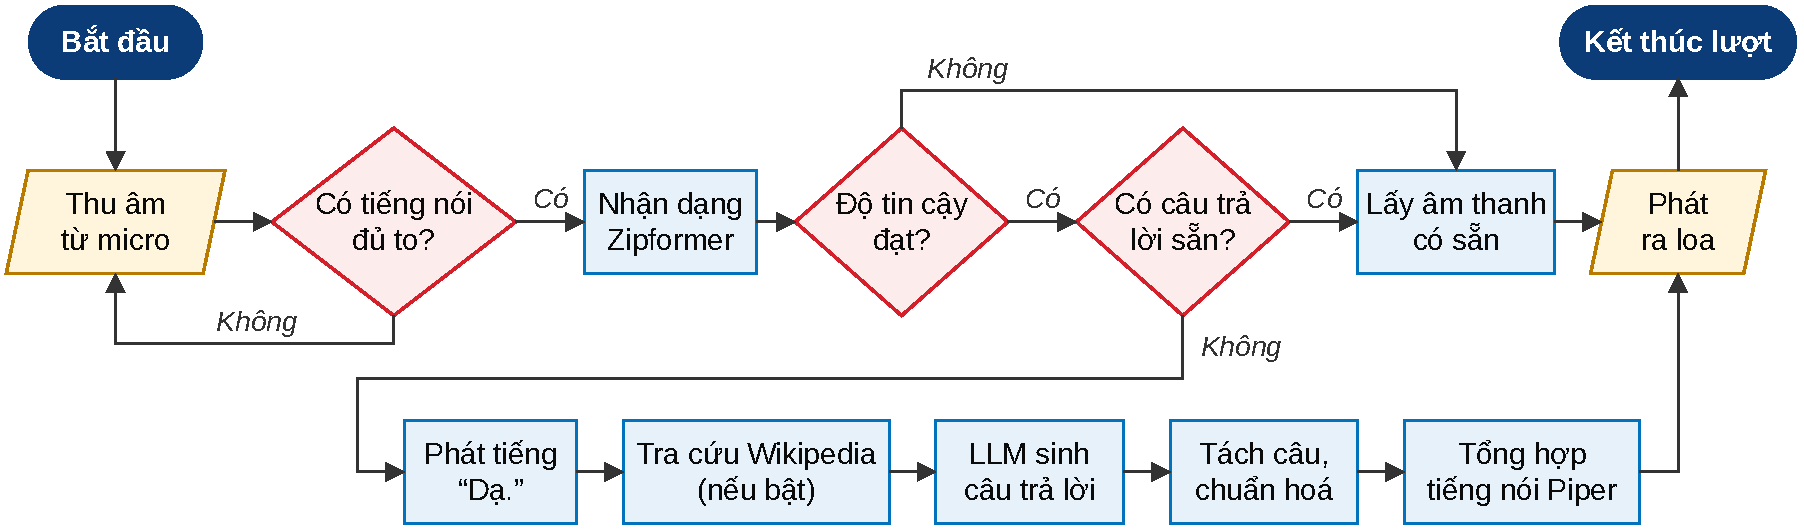
\includegraphics[width=\textwidth]{luu_do.pdf}
\caption{Lưu đồ xử lý một lượt hỏi. Câu không đủ tin cậy và câu có sẵn đều lấy âm thanh tổng hợp sẵn (lần lượt là lời đề nghị nói lại và câu trả lời), không qua LLM. Các câu còn lại qua tra cứu, LLM và TTS theo dòng, nên tiếng đầu có thể phát trước khi LLM viết xong. Cùng lưu đồ chạy trên Pi 5 (âm thanh ở lõi 3, phần còn lại ở lõi 0 đến 2) và trên Fold7 (LLM ở NPU).}\label{fig:arch}
\end{figure*}

Tra cứu dùng 200.000 bài Wikipedia tiếng Việt (1,7 triệu đoạn) lưu trong SQLite FTS5~\cite{fts5}, xếp hạng BM25, chèn đoạn trích 240 ký tự vào câu hỏi theo cách làm của RAG~\cite{rag}. Tệp chỉ mục 1,4\,GB dùng chung cho Pi và điện thoại.

\subsection{LLM và lượng tử hoá}
LLM chạy bằng llama.cpp~\cite{llamacpp} (cùng một phiên bản mã nguồn trên mọi thiết bị). Chúng tôi tinh chỉnh LoRA~\cite{lora} các mô hình Qwen3.5~\cite{qwen} bản 0,8 tỉ và 2 tỉ tham số trên 3.464 cặp hỏi đáp tiếng Việt tự sinh và tự kiểm tra, để câu trả lời ngắn và dễ nghe. Trên Cortex-A76, định dạng Q4\_0 được llama.cpp đóng gói lại thành khối 4$\times$4 phù hợp lệnh dotprod, nhờ đó nhanh hơn Q4\_K\_M dù cùng 4 bit (Bảng~\ref{tab:quant}).

\subsection{Giảm độ trễ}
Với câu qua LLM, thời gian từ lúc nói xong tới lúc nghe câu trả lời thật là
\begin{equation}
\begin{split}
T ={}& T_{\text{ngắt}} + T_{\text{STT}} + T_{\text{tra cứu}}\\
&+ T_{\text{TTFT}} + T_{\text{câu đầu}} + T_{\text{TTS}}.
\end{split}
\end{equation}
Từ (1) có ba biện pháp. Một là đường nhanh: 149 cặp hỏi đáp có sẵn, khớp sau khi bỏ dấu câu, phát âm thanh đã tổng hợp sẵn nên loại bỏ cả bốn số hạng cuối. Hai là cắt câu đầu sớm sau 3 từ thay vì 5 từ, giảm $T_{\text{câu đầu}}$ và $T_{\text{TTS}}$. Ba là xác nhận tức thì: tiếng ``Dạ.'' phát ngay khi có chữ. Biện pháp cuối chỉ giảm độ trễ cảm nhận và không làm câu trả lời đến sớm hơn, nên chúng tôi báo hai chỉ số riêng.

\subsection{Triển khai trên Android}
Chuyển đường ống sang điện thoại gặp ba vấn đề kỹ thuật. Thư viện OpenCL và FastRPC của nhà sản xuất chỉ thấy được từ tiến trình của ứng dụng, nên \texttt{llama-server} được nạp ngay trong tiến trình qua JNI thay vì chạy như chương trình con. SQLite của Android không có FTS5, nên ứng dụng dùng bản SQLite đóng gói riêng. Tệp mô hình đặt trong vùng riêng của ứng dụng để bộ nạp đọc được. Phần tách câu, chuẩn hoá và đường nhanh được viết lại bằng Kotlin từ bản Python trên Pi để hai nền tảng cho cùng hành vi.

\subsection{Chống nhận nhầm tiếng ồn}
Khi để yên, Zipformer từng chép một đoạn ồn 1,3\,s (RMS 0,003) thành một câu có nghĩa. Chúng tôi tắt AGC của micro và chỉ nhận đoạn thoả
\begin{equation}
\text{RMS}(x) \ge \max(0{,}008;\ 2{,}5\,\hat{n}),
\end{equation}
trong đó $\hat{n}$ là mức nền đo liên tục. Câu một từ bị bỏ qua nếu không trúng đường nhanh.

\subsection{Thời gian thực trên Pi}
PREEMPT\_RT~\cite{preemptrt} được dựng bằng Yocto~\cite{yocto}. Tiến trình âm thanh chạy trên lõi 3 đã cô lập (\texttt{isolcpus=3 nohz\_full=3 rcu\_nocbs=3}), SCHED\_FIFO mức 80, khoá bộ nhớ. STT, LLM và TTS ở lõi 0 đến 2.

\subsection{Thẻ an toàn đã kiểm duyệt}
Mô hình nhỏ bịa 12\% đến 52\% số câu trả lời (Mục~3.3), chấp nhận được với câu hỏi kiến thức nhưng không được với ``con tôi bị rắn cắn''. Vì vậy câu hỏi khẩn cấp được trả lời bằng thẻ viết sẵn chứ không do LLM viết. Bộ 42 thẻ (24 sơ cứu, 10 thiên tai, 8 sinh tồn, trung bình 75 từ) được viết lại bằng lời của nhóm từ 42 nguồn: hướng dẫn của Cục Quản lý đê điều và Phòng, chống thiên tai, Bộ Y tế, Quyết định 2024/QĐ-TTg về số 112, tài liệu thuộc phạm vi công cộng của Ready.gov (bản tiếng Việt), CDC, NWS, và MedlinePlus, WHO, Hội Chữ Thập Đỏ Úc. Câu nào không có trong nguồn đều bị xoá khỏi thẻ. Khi rà soát, nhóm phát hiện bản dịch Ready.gov ghi nhầm ngưỡng bỏ thức ăn là 40 độ C thay vì 40 độ F, nên không dùng con số đó.

Bộ khớp giữ dấu tiếng Việt, vì bỏ dấu thì ``bất tỉnh'' trùng ``bật tính'' và ``đuối nước'' trùng ``dưới nước''. Một thẻ được chọn khi câu chứa một cụm từ khoá của nó hoặc một tổ hợp từ (``rắn'' và ``cắn'' ở bất kỳ đâu trong câu); thẻ cụ thể hơn được ưu tiên. Câu hỏi kiến thức như ``lũ quét hình thành thế nào'' được để cho LLM. Câu khẩn cấp không có thẻ nhận câu trả lời cố định: chưa có hướng dẫn đã kiểm duyệt, hãy gọi 115 hoặc 112. Luật nằm trong cùng tệp dữ liệu nên bản Python trên Pi và bản Kotlin trên điện thoại cho kết quả giống hệt nhau trên 918 câu thử; mỗi câu khớp mất khoảng 0,1\,ms.

\subsection{Tính năng và ưu điểm của thiết kế}
Bảng~\ref{tab:feat} liệt kê tính năng đã hoàn thành trên hai nền tảng, Hình~\ref{fig:dash} là bảng điều khiển web. Thiết kế có bốn ưu điểm chính. Thứ nhất, toàn bộ xử lý nằm trên thiết bị, không có lời gọi mạng ra ngoài, nên giọng nói không rời máy và hệ thống vẫn chạy khi mất Internet. Thứ hai, mỗi khối (STT, LLM, TTS, tra cứu, bộ xử lý) chọn được bằng cấu hình, nên cùng một đường ống chạy trên Pi và trên điện thoại, và có thể đổi mô hình khi có bản tốt hơn. Thứ ba, mọi lượt đều ghi mốc thời gian từng chặng, nên mỗi tối ưu trong bài đều có số đo trước và sau. Thứ tư, câu có sẵn và câu hỏi tự do đi hai nhánh riêng, nên câu hỏi thường gặp được trả lời gần như tức thì mà không làm mất khả năng trả lời câu hỏi mới.

\begin{table}[t]\centering\small
\caption{Tính năng đã hoàn thành. $\checkmark$: có; $\times$: không có.}\label{tab:feat}
\setlength{\tabcolsep}{3pt}
\begin{tabular}{@{}L{58mm}cc@{}}\toprule
Tính năng & Pi 5 & Fold7\\\midrule
Hỏi đáp tiếng Việt offline & $\checkmark$ & $\checkmark$\\
Đường nhanh cho câu hỏi có sẵn & $\checkmark$ & $\checkmark$\\
Tra cứu Wikipedia offline, bật tắt được & $\checkmark$ & $\checkmark$\\
Xác nhận tức thì ``Dạ.'' & $\checkmark$ & $\checkmark$\\
Chạm để nói, tự dừng khi im lặng & $\checkmark$ & $\checkmark$\\
Lọc tiếng ồn, bỏ câu một từ & $\checkmark$ & $\checkmark$\\
Đề nghị nói lại theo độ tin cậy & $\checkmark$ & $\times$\\
Chọn CPU, GPU hoặc NPU cho LLM & $\times$ & $\checkmark$\\
Bảng điều khiển đo từng chặng & $\checkmark$ & $\times$\\
Điện thoại làm micro, loa cho Pi & $\checkmark$ & $\checkmark$\\
Lõi âm thanh thời gian thực & $\checkmark$ & $\times$\\
Thẻ sơ cứu, thiên tai có nguồn & $\checkmark$ & $\checkmark$\\\bottomrule
\end{tabular}
\end{table}

\begin{figure}[t]
\centering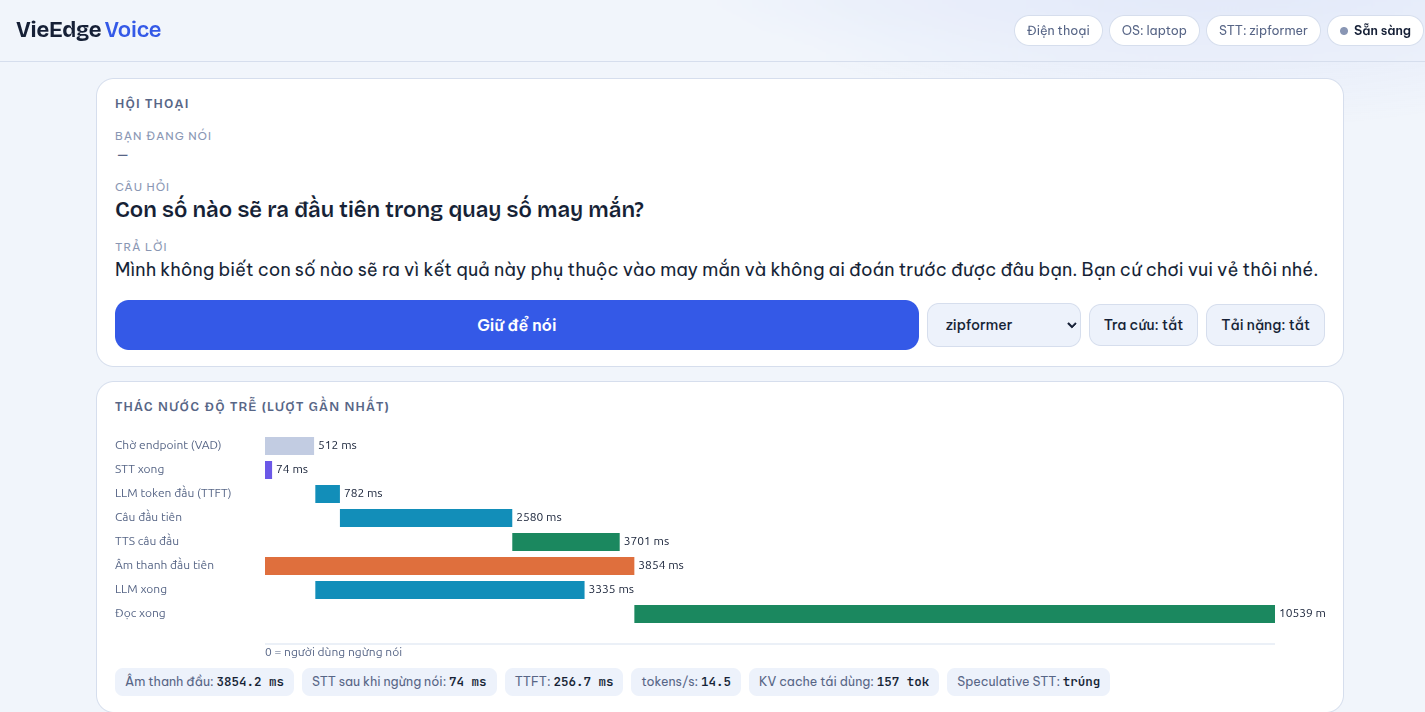
\includegraphics[width=\columnwidth]{dashboard.png}
\caption{Bảng điều khiển web: câu hỏi, câu trả lời, nút giữ để nói, công tắc tra cứu và biểu đồ thời gian từng chặng của lượt gần nhất. Ảnh chụp khi chạy minh hoạ trên máy tính xách tay; số trên ảnh là của lần chạy đó, không phải số đo trên Pi hay Fold7.}\label{fig:dash}
\end{figure}

\subsection{Giao thức đo}
Mọi độ trễ tính từ lúc người dùng nói xong và gồm cả thời gian chờ ngắt câu. Câu hỏi là 12 đến 16 câu giọng đọc tổng hợp, khác giọng trợ lý, phát qua cùng một bộ công cụ cho mọi cấu hình; trên điện thoại đưa trực tiếp vào ứng dụng, trên Pi nạp từ tệp. ``Tiếng đầu'' là âm thanh đầu tiên nghe được, ``câu trả lời thật'' là lúc bắt đầu đọc nội dung trả lời. Chúng tôi báo trung vị p50 và p95, khoảng tin cậy 95\% của trung vị bằng bootstrap (10.000 lần lấy mẫu), và kiểm định Wilcoxon cặp đôi khi so sánh cùng bộ câu. WER đo trên VIVOS~\cite{vivos} với cùng một chương trình. Độ chính xác LLM đo bằng Global-MMLU tiếng Việt~\cite{gmmlu} ($n=400$, sai số $\pm 2{,}5$ điểm) và bằng giám khảo là mô hình lớn hơn trên 345 câu.

\section{Kết quả và thảo luận}
\subsection{Chỉ tiêu và kết quả}
Bảng~\ref{tab:target} đối chiếu kết quả với chỉ tiêu đặt ra trong đề xuất ban đầu. Ba chỉ tiêu đạt, một chỉ tiêu chưa đạt, và phần chạy trên điện thoại vượt kế hoạch. Câu trả lời thật chưa có chỉ tiêu riêng; p95 của nó vẫn trên 1,5\,s ở cả hai nền tảng.

\begin{table}[t]\centering\small
\caption{Chỉ tiêu trong đề xuất và kết quả đo.}\label{tab:target}
\setlength{\tabcolsep}{3pt}
\begin{tabular}{@{}L{27mm}L{36mm}l@{}}\toprule
Chỉ tiêu & Kết quả & Đánh giá\\\midrule
Tiếng đầu p95 dưới 1,5\,s & Pi 1,15\,s; Fold7 1,24\,s & Đạt\\
Không xrun & 0 (chưa thử loa, micro USB) & Đạt\\
STT trên NPU Hailo-8L & cosine 0,84, dưới ngưỡng 0,9 & Chưa đạt\\
Hoàn toàn offline & không cần mạng & Đạt\\
Chạy trên điện thoại & 1,53\,s, có tra cứu & Vượt\\\bottomrule
\end{tabular}
\end{table}

\subsection{Nhận dạng giọng nói}
Bảng~\ref{tab:wer} so sánh trực tiếp trên cùng tập câu. Zipformer sai ít hơn khoảng ba lần so với PhoWhisper-tiny khi sạch và bốn lần ở nhiễu 5\,dB. Trên 300 câu VIVOS, WER của Zipformer là 0,041, mỗi câu tốn 29\,ms trên máy tính xách tay (hệ số thời gian thực 0,008). PhoWhisper-tiny dùng cửa sổ 30\,s đạt 0,114, tốt hơn con số 0,158 của cửa sổ 10\,s trong bảng; chúng tôi chọn 10\,s vì đó là bản biên dịch được cho Hailo. Trên điện thoại, 12 câu tổng hợp cho WER 0,257, so với 0,250 của máy tính xách tay trên đúng các tệp đó, nên bản Android không kém trong phạm vi mẫu nhỏ này.

\begin{table}[t]\centering\small
\caption{WER (càng thấp càng tốt). Whisper và PhoWhisper bản tiny; cùng tập câu cho hai cột phải; câu TTS: $n=120$.}\label{tab:wer}
\setlength{\tabcolsep}{4pt}
\begin{tabular}{@{}lrrr@{}}\toprule
Điều kiện & Whisper & PhoWhisper & Zipformer\\\midrule
VIVOS sạch & 0,529 & 0,158 & \textbf{0,046}\\
VIVOS 10\,dB & & 0,169 & \textbf{0,040}\\
VIVOS 5\,dB & & 0,224 & \textbf{0,059}\\
Câu TTS & & 0,312 & \textbf{0,189}\\\bottomrule
\end{tabular}
\end{table}

\begin{table}[t]\centering\small
\caption{Lượng tử 0,8 tỉ tham số: tốc độ đo trên Pi 5 (Pi OS, 3 luồng); MCQ $n=400$, ba định dạng 4 bit không phân biệt được trong sai số.}\label{tab:quant}
\begin{tabular}{@{}lrrr@{}}\toprule
Định dạng & Nạp (t/s) & Sinh (t/s) & MCQ\\\midrule
Q4\_K\_M & 87,9 & 16,2 & 0,333\\
\textbf{Q4\_0} & \textbf{125,3} & \textbf{18,2} & 0,308\\
IQ4\_NL & 96,0 & 17,6 & 0,340\\
Q8\_0 & chưa đo & chưa đo & 0,393\\\bottomrule
\end{tabular}
\end{table}

Điểm tin cậy của Zipformer phân biệt được câu nhận sai với AUROC 0,84; ngưỡng $-0{,}20$ từ chối 4,7\% số câu. Trên giọng tổng hợp, cổng này chặn 4 trong 16 câu ở Yocto và 5 trong 16 câu ở Pi OS, và các lượt đó được yêu cầu nói lại; chúng tôi chưa đo được bao nhiêu trong số này thực sự bị nghe sai.

\subsection{Chất lượng câu trả lời}
Điểm giám khảo thang 5 là 3,63 với mô hình 0,8 tỉ và 4,17 với mô hình 2 tỉ, tỉ lệ bịa của mô hình 2 tỉ là 0,12. Khi câu hỏi đi qua nhận dạng giọng nói, tỉ lệ bịa của mô hình 0,8 tỉ tăng lên 0,52; bật tra cứu đưa nó về 0,30. Lỗi nhận dạng là nguồn mất chính xác lớn nhất: điểm giảm từ 3,64 trên câu gõ xuống 2,73 trên câu qua Zipformer, với câu hỏi giọng tổng hợp có WER 0,19.

\subsection{Thời gian đi đâu}\label{sec:latency}
Hình~\ref{fig:stages} tách trung vị từng chặng của các lượt thực sự qua LLM. Trên Pi, phần lớn thời gian nằm ở LLM viết đủ câu đầu và TTS đọc câu đó, không phải ở token đầu tiên. Trên Fold7 hai chặng này giảm mạnh và chặng lớn nhất là 0,63\,s gồm chờ ngắt câu, STT và tra cứu, trong đó token đầu chỉ mất 0,20\,s. Tăng tốc LLM thêm nữa vì vậy khó còn tác dụng lớn.

\begin{figure}[t]
\centering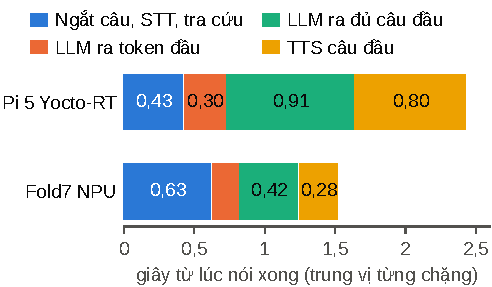
\includegraphics[width=\columnwidth]{stages.pdf}
\caption{Thời gian tới câu trả lời thật theo chặng. Pi: 0,8 tỉ, tắt tra cứu, câu đầu 5 từ ($n=12$). Fold7: 2 tỉ, NPU, bật tra cứu, câu đầu 3 từ ($n=13$). Hai cấu hình khác nhau, hình cho thấy cơ cấu thời gian chứ không phải so sánh thiết bị thuần tuý.}\label{fig:stages}
\end{figure}

\begin{figure}[t]
\centering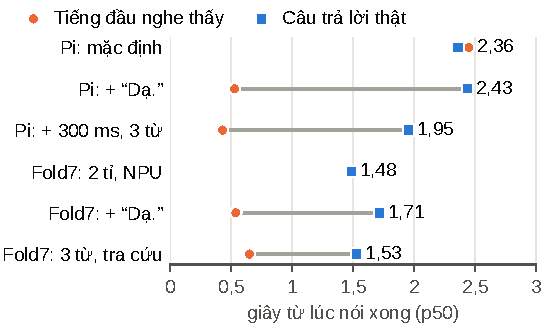
\includegraphics[width=\columnwidth]{latency.pdf}
\caption{Xác nhận tức thì kéo tiếng đầu xuống khoảng 0,5\,s nhưng câu trả lời thật không sớm hơn. Số bên phải là câu trả lời thật (p50, 12 đến 13 lượt).}\label{fig:latency}
\end{figure}

Hình~\ref{fig:latency} và Bảng~\ref{tab:abl} cho kết quả bật tắt từng biện pháp. Cắt câu đầu từ 5 xuống 3 từ giảm p50 từ 2,03\,s xuống 1,60\,s và p95 từ 3,51\,s xuống 2,38\,s; khoảng tin cậy của p50 còn chồng nhau nên đây là xu hướng, chưa phải kết luận chắc chắn. Tăng luồng TTS và rút thời gian ngắt câu còn 300\,ms không tạo khác biệt vượt khoảng tin cậy, nên cấu hình mặc định giữ 400\,ms để tránh cắt ngang người nói chậm. Giọng \texttt{x\_low} nhanh hơn giọng chuẩn khoảng 0,2\,s (1,27\,s so với 1,48\,s, cùng tắt xác nhận) nhưng chất giọng thấp hơn. Đường nhanh trên Pi trả lời câu có sẵn sau 0,52\,s, gần bằng thời gian chờ ngắt câu, và không trả lời nhầm bằng câu có sẵn cho câu nào trong 345 câu hỏi kiến thức của tập thử.

\begin{table}[t]\centering\small
\caption{Bật tắt trên Fold7 (2 tỉ, NPU, tra cứu và ``Dạ.'' bật, $n=12$ đến 13). Cấu hình: số từ câu đầu, luồng TTS, thời gian ngắt câu (ms). KTC: khoảng tin cậy 95\% của p50 câu thật. Mặc định là dòng in đậm.}\label{tab:abl}
\setlength{\tabcolsep}{3pt}
\begin{tabular}{@{}lrrr@{}}\toprule
Cấu hình & Tiếng đầu & Câu thật & KTC\\\midrule
5 từ, 3 luồng, 400 & 0,66 & 2,03 & [1,47; 2,19]\\
3 từ, 3 luồng, 400 & 0,66 & 1,60 & [1,39; 1,70]\\
\textbf{3 từ, 4 luồng, 400} & \textbf{0,65} & \textbf{1,53} & [1,47; 1,78]\\
3 từ, 4 luồng, 300 & 0,57 & 1,55 & [1,40; 1,92]\\\bottomrule
\end{tabular}
\end{table}

\subsection{So sánh nền tảng}\label{sec:platform}
Hình~\ref{fig:platform} cho thấy NPU Hexagon nạp prompt nhanh gấp 16 lần CPU Pi 5 trên cùng tệp mô hình, trong khi CPU điện thoại sinh token nhanh nhất. Đây là lý do tra cứu gần như miễn phí trên điện thoại. Thời gian tra cứu là 96\,ms (p50) và prompt tăng từ 25 lên 107 token, nhưng câu trả lời thật chỉ chậm thêm 0,06\,s (1,69\,s so với 1,75\,s). Cùng tính năng trên Pi làm chậm thêm 1,4 đến 2,8\,s. GPU Adreno sinh nhanh hơn trong ứng dụng (2 tỉ: 36 so với 26 token/s) nhưng thời gian trả lời gần bằng NPU và nạp mô hình lâu hơn (14 đến 24\,s so với 6 đến 8\,s).

\begin{figure}[t]
\centering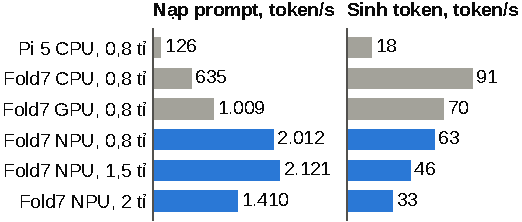
\includegraphics[width=\columnwidth]{platform.pdf}
\caption{\texttt{llama-bench} (prompt 128, sinh 64 token), bản Q4\_0. NPU mạnh ở nạp prompt, CPU mạnh ở sinh token: tra cứu rẻ trên NPU vì prompt dài được nạp rất nhanh.}\label{fig:platform}
\end{figure}

Bảng~\ref{tab:model} cho thấy đánh đổi giữa mô hình và bộ xử lý khi tắt xác nhận và tra cứu. Mô hình 0,8 tỉ trả lời nhanh hơn 2 tỉ khoảng 0,3\,s nhưng điểm giám khảo thấp hơn 0,54 điểm. Với một trợ lý hỏi đáp, chúng tôi chọn 2 tỉ trên NPU làm mặc định: chất lượng cao hơn và nạp mô hình nhanh, đổi lại p95 kém nhất trong bảng (3,22\,s). GPU ổn định hơn ở p95 nhưng nạp lâu. Số lượt ít nên thứ tự giữa các dòng cần được xem như xu hướng.

\begin{table}[t]\centering\small
\caption{Fold7 theo mô hình và bộ xử lý (tắt xác nhận, tắt tra cứu, 12 đến 22 lượt). Giọng \texttt{x\_low} chất lượng thấp hơn giọng chuẩn. Điểm giám khảo đo riêng trên máy tính xách tay.}\label{tab:model}
\setlength{\tabcolsep}{3.5pt}
\begin{tabular}{@{}lrrrr@{}}\toprule
Cấu hình & p50 (s) & p95 (s) & token/s & Điểm\\\midrule
0,8 tỉ, NPU & 1,19 & 1,71 & 27 & 3,63\\
0,8 tỉ, GPU & 1,22 & 1,48 & 60 & 3,63\\
2 tỉ, GPU & 1,31 & 1,74 & 36 & 4,17\\
\textbf{2 tỉ, NPU} & \textbf{1,48} & \textbf{3,22} & \textbf{26} & \textbf{4,17}\\
2 tỉ, NPU, \texttt{x\_low} & 1,27 & 1,83 & 26 & 4,17\\\bottomrule
\end{tabular}
\end{table}

\subsection{Điện thoại làm micro và loa cho Pi}
Ở chế độ máy chủ, điện thoại gửi micro sang Pi và phát lại tiếng trả lời qua WebSocket trong cùng mạng Wi-Fi. Đo bằng một máy khách giả lập qua mạng thật, câu có sẵn nghe thấy sau khoảng 0,59\,s, gồm 0,15\,s mạng và bộ đệm. Câu qua LLM có tiếng ``Dạ.'' lúc 0,59\,s và câu trả lời thật lúc 1,6 đến 1,8\,s; bật tra cứu thì 3,0 đến 4,5\,s. Tiến trình âm thanh trên lõi 3 không có xrun trong cả phiên. Chế độ này cho phép Pi phục vụ không cần loa, micro USB, nhưng vẫn cần mạng nội bộ, nên chế độ chạy trọn vòng trên điện thoại là cấu hình mặc định.

\subsection{Pi OS và Yocto-RT}\label{sec:os}
Bảng~\ref{tab:os} dùng cùng bo mạch, cùng chương trình đo, cùng mô hình Q4\_0. Yocto-RT giảm đỉnh jitter khi tải nặng từ 105 xuống 85\,µs trong 5 phút và từ 127 xuống 92\,µs trong 30 phút (Hình~\ref{fig:jitter}, 1,8 triệu mẫu), còn p99 đến p99,99 gần như bằng nhau. Yocto dùng ít RAM hơn sau khởi động. Về độ trễ trả lời khi yên, trung vị của Pi OS thấp hơn 0,42\,s, nhưng so cặp trên cùng 16 câu thì chênh lệch trung vị chỉ 0,06\,s (khoảng tin cậy $-0{,}08$ đến $0{,}59$\,s, Wilcoxon $p=0{,}40$). Các số này gồm cả lượt yêu cầu nói lại; chỉ xét lượt qua LLM thì trung vị là 1,85\,s và 2,44\,s, so cặp 11 câu cho $p=0{,}83$. Với cỡ mẫu này chúng tôi không thể khẳng định hệ nào nhanh hơn. Kết luận trung thực là Yocto-RT mang lại sự cô lập và ảnh gọn, không phải tốc độ suy luận.

\begin{table}[t]\centering\small
\caption{Pi OS nguyên bản (O0) và Yocto-RT (O4) trên cùng Pi 5, LLM 0,8 tỉ Q4\_0. Yocto 30 phút đo bản Q4\_K\_M.}\label{tab:os}
\setlength{\tabcolsep}{3pt}
\begin{tabular}{@{}lrr@{}}\toprule
Chỉ số & Pi OS & Yocto-RT\\\midrule
Đỉnh jitter, rảnh, 5 ph (µs) & 33 & \textbf{13}\\
Đỉnh jitter, tải nặng, 5 ph (µs) & 105 & \textbf{85}\\
Đỉnh jitter, tải nặng, 30 ph (µs) & 127 & \textbf{92}\\
Trả lời, yên, p50 (s) & 1,60 & 2,02\\
Trả lời, yên, p95 (s) & 3,62 & 3,78\\
Trả lời, nhiễu 4 lõi, p50 (s) & 9,27 & \textbf{6,51}\\
RAM sau khởi động (MB) & 442-538$^{\dagger}$ & \textbf{285}\\
Công suất PMIC, yên (W) & 3,03 & \textbf{2,78}\\
Xrun trên giờ & 0 & 0\\\bottomrule
\end{tabular}\\[1pt]
{\footnotesize $^{\dagger}$ đo ở cấu hình O1.}
\end{table}

\begin{figure}[t]
\centering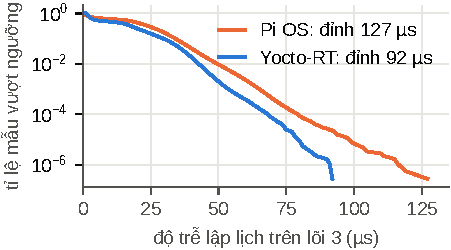
\includegraphics[width=\columnwidth]{jitter.pdf}
\caption{Đuôi jitter lõi 3 khi tải nặng, 30 phút, 1 kHz, SCHED\_FIFO 80. Khác biệt nằm ở phần đuôi rất hiếm, thân phân phối gần như trùng nhau.}\label{fig:jitter}
\end{figure}

\subsection{Nhiệt và công suất}
Chạy liên tục 7,5 phút (62 lượt), NPU cao nhất 65\,°C và tốc độ giữ 25,3 token/s từ quý đầu tới quý cuối, tức không có dấu hiệu hạ xung (Hình~\ref{fig:soak}). Khi rút sạc, 78 lượt trong 9,4 phút tiêu thụ 2,2 đến 3,3\,W cho cả máy kể cả màn hình, tương đương 16 đến 24\,J mỗi lượt; chưa tách riêng được NPU. Pi 5 ở trên cho 2,78\,W theo ước lượng PMIC của bo mạch, chưa tính loa và micro, nên hai con số không cùng phạm vi.

\begin{figure}[t]
\centering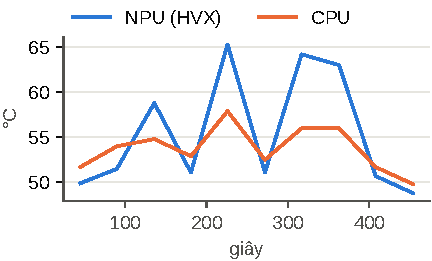
\includegraphics[width=\columnwidth]{soak.pdf}
\caption{Nhiệt độ Fold7 trong 62 lượt liên tục, mẫu mỗi 45\,s. Nhiệt dao động theo tải nhưng tốc độ sinh token không đổi.}\label{fig:soak}
\end{figure}

\subsection{Kịch bản an toàn khi mất sóng}\label{sec:safety}
Bảng~\ref{tab:safety} cho kết quả bộ khớp. Tập phát triển được dùng để chỉnh luật nên kết quả 100\% của nó không phải số đo độc lập. Tập độc lập đầu tiên cho thấy luật cụm từ ban đầu chỉ chọn đúng 60\% vì người hỏi diễn đạt rất khác nhau; nhóm thêm luật tổ hợp từ, khoá luật lại (ghi mã băm của tệp), rồi mới viết tập độc lập thứ hai. Trên tập này, 94\% câu chọn đúng thẻ và không câu nào bị chọn sai thẻ; 5 câu bị sót và sẽ đi sang LLM. Trong 30 câu thường được viết cố ý để gài bẫy (``bão giá'', ``lũ trẻ'', ``cháy hàng'', ``mèo cào ghế''), 7 câu bị kích hoạt nhầm. Khi các câu này được đọc bằng giọng tổng hợp chất lượng thấp rồi qua Zipformer, lỗi nhận dạng lên 35\% số từ và tỉ lệ đúng thẻ giảm còn 48\%; điểm yếu nằm ở khâu nghe chứ không ở khâu khớp. Trên Fold7 ở chế độ máy bay, 16 câu khẩn cấp phát hai lần đều nhận đúng thẻ (32/32); tiếng đầu tính từ lúc nói xong là 0,83\,s ở lần đầu và 0,50\,s khi âm thanh đã có trong bộ nhớ đệm. Bản Kotlin cho kết quả giống hệt bản Python trên 918 câu khi chạy ngay trên máy.

Một hướng nhóm đã thử là để LLM chọn thẻ, với đầu ra bị ràng buộc vào danh sách mã thẻ. Mô hình 2 tỉ tham số chỉ chọn đúng 2 trên 126 câu của tập phát triển và chọn nhầm một thẻ cho 140 trên 345 câu hỏi chung, nên không dùng.

\begin{table}[t]\centering\small
\caption{Bộ khớp thẻ an toàn. Có thẻ: số câu đúng thẻ (sót; sai thẻ). Không thẻ: số câu nhận câu ``gọi 115''. Thường: số câu bị kích hoạt nhầm. Độc lập 1 chạy luật ban đầu; độc lập 2 chạy luật đã khoá trước khi viết câu.}\label{tab:safety}
\setlength{\tabcolsep}{1.5pt}
\begin{tabular}{@{}lrrr@{}}\toprule
Tập câu & Có thẻ & Không thẻ & Thường\\\midrule
Phát triển & 126/126 & 20/20 & 0/370\\
Độc lập 1 & 50/84 (29; 5) & 12/20 & 1/30\\
\textbf{Độc lập 2} & \textbf{79/84} (5; 0) & 16/20 & 7/30\\
Độc lập 2 qua STT & 40/84 (41; 3) & 9/20 & 3/30\\\bottomrule
\end{tabular}
\end{table}

\subsection{Những gì đã thử mà không hiệu quả}\label{sec:negative}
Encoder PhoWhisper-tiny biên dịch được cho Hailo-8L (HEF 19 đến 20\,MB) nhưng cosine với ONNX chỉ 0,842 khi lượng tử thường và 0,655 sau tinh chỉnh lượng tử 6 epoch, dưới ngưỡng 0,9 chúng tôi đặt ra, nên không đưa vào đường ống và chưa có WER trên Hailo thật. Giải mã suy đoán~\cite{speculative} không nhanh hơn (13,9 so với 14,3 token/s). Cửa sổ STT thích ứng làm WER tăng gấp đôi (0,158 lên 0,354). LoRA huấn luyện trên câu có nhiễu nhận dạng tăng 0,14 điểm trên câu qua STT nhưng mất 0,16 điểm trên câu sạch. Lượng tử Q3\_K\_M làm MCQ của mô hình 2 tỉ giảm từ 0,445 (Q4\_K\_M) xuống 0,37.

\subsection{Hạn chế}
Toàn bộ độ trễ đo bằng giọng đọc tổng hợp, chưa có người nói thật; Zipformer sai 19\% trên giọng này so với 4\% trên VIVOS, nên kết quả chất lượng có thể khác với người dùng thật. Mỗi cấu hình chỉ 12 đến 16 lượt, đủ thấy chênh lệch lớn nhưng không đủ cho chênh lệch dưới khoảng 10\%. Giám khảo là mô hình lớn, không phải người. Zipformer-vi có giấy phép phi thương mại và VIVOS có thể trùng một phần dữ liệu huấn luyện của nó. Các thẻ an toàn chưa được người có chuyên môn y tế duyệt và câu thử do nhóm viết, nên trước khi đưa cho người dùng thật cần cả hai việc này. Bước có giá trị nhất tiếp theo là thu một tập giọng người trên micro điện thoại trong phòng thật, vì nó biến các số ở đây từ mô phỏng thành đo thực tế.

\section{Kết luận}
VieEdge-Voice cho thấy hỏi đáp giọng nói tiếng Việt chạy được offline trọn vòng trên thiết bị biên. Trên Pi 5, câu có sẵn được trả lời sau 0,52\,s và câu qua LLM sau khoảng 2 đến 2,4\,s; trên Fold7, mô hình 2 tỉ tham số kèm tra cứu trả lời sau 1,53\,s. Khi muốn nhanh hơn, nên đo cơ cấu thời gian trước: chờ ngắt câu và câu đầu chiếm nhiều hơn token đầu tiên. Hệ điều hành thời gian thực đáng dùng khi cần cô lập lõi âm thanh, không phải để tăng tốc suy luận. Với câu hỏi khẩn cấp, thẻ có nguồn đáng tin hơn câu do mô hình nhỏ sinh ra, và bộ khớp đơn giản nhưng được đo trên tập độc lập tốt hơn hẳn việc để LLM tự chọn. Hướng tiếp theo là đo với giọng người và ngắt câu theo ngữ nghĩa để giảm thời gian chờ.

\balance
\section{Tài liệu tham khảo}
\vspace{-20pt}
{\small\setlength{\parskip}{0pt}\raggedright
\begin{thebibliography}{99}\setlength{\itemsep}{1pt}
\bibitem{stivers} T. Stivers et al., Universals and cultural variation in turn-taking in conversation, Proceedings of the National Academy of Sciences, 106(26), pp. 10587-10592, 2009.
\bibitem{whisper} A. Radford, J. W. Kim, T. Xu, G. Brockman, C. McLeavey, I. Sutskever, Robust speech recognition via large-scale weak supervision, Proceedings of ICML, PMLR 202, pp. 28492-28518, 2023.
\bibitem{phowhisper} T.-T. Le, L. T. Nguyen, D. Q. Nguyen, PhoWhisper: automatic speech recognition for Vietnamese, ICLR Tiny Papers, 2024.
\bibitem{chipchat} T. Likhomanenko et al., ChipChat: low-latency cascaded conversational agent in MLX, arXiv:2509.00078, 2025.
\bibitem{melt} S. Laskaridis, K. Katevas, L. Minto, H. Haddadi, MELTing point: mobile evaluation of language transformers, Proceedings of ACM MobiCom, pp. 890-907, 2024.
\bibitem{silero} Silero Team, Silero VAD, github.com/snakers4/silero-vad.
\bibitem{zipformer} Z. Yao et al., Zipformer: a faster and better encoder for automatic speech recognition, Proceedings of ICLR, 2024.
\bibitem{zipvi} hynt, Zipformer-30M-RNNT-6000h, huggingface.co/hynt/Zipformer-30M-RNNT-6000h.
\bibitem{sherpa} k2-fsa, sherpa-onnx, github.com/k2-fsa/sherpa-onnx.
\bibitem{piper} Rhasspy, Piper text-to-speech, github.com/rhasspy/piper.
\bibitem{vits} J. Kim, J. Kong, J. Son, Conditional variational autoencoder with adversarial learning for end-to-end text-to-speech, Proceedings of ICML, PMLR 139, pp. 5530-5540, 2021.
\bibitem{fts5} SQLite Consortium, FTS5 extension, sqlite.org/fts5.html.
\bibitem{rag} P. Lewis et al., Retrieval-augmented generation for knowledge-intensive NLP tasks, Proceedings of NeurIPS, 2020.
\bibitem{llamacpp} G. Gerganov et al., llama.cpp, github.com/ggml-org/llama.cpp, commit 7fe450e19.
\bibitem{lora} E. J. Hu et al., LoRA: low-rank adaptation of large language models, Proceedings of ICLR, 2022.
\bibitem{qwen} Qwen Team, Qwen3.5 model cards, huggingface.co/Qwen.
\bibitem{preemptrt} F. Reghenzani, G. Massari, W. Fornaciari, The real-time Linux kernel: a survey on PREEMPT\_RT, ACM Computing Surveys, 52(1), article 18, 2019.
\bibitem{yocto} The Yocto Project, Reference manual, docs.yoctoproject.org.
\bibitem{vivos} H.-T. Luong, H.-Q. Vu, A non-expert Kaldi recipe for Vietnamese speech recognition system, Proceedings of the WLSI/OIAF4HLT Workshop at COLING, Osaka, pp. 51-55, 2016.
\bibitem{gmmlu} S. Singh et al., Global MMLU: understanding and addressing cultural and linguistic biases in multilingual evaluation, Proceedings of ACL, 2025.
\bibitem{speculative} Y. Leviathan, M. Kalman, Y. Matias, Fast inference from transformers via speculative decoding, Proceedings of ICML, PMLR 202, pp. 19274-19286, 2023.
\end{thebibliography}}

\vspace{4pt}
\noindent\begin{minipage}{\columnwidth}\setlength{\parskip}{0pt}
\textbf{Tác giả chịu trách nhiệm bài viết:}\\
Họ tên: \svmot\\
Đơn vị: \khoa, \truong\\
Email: \emailmot
\end{minipage}
\end{document}
